\documentclass[conference]{IEEEtran}
\usepackage{graphicx}
\usepackage{cite}
\usepackage{amsmath, amssymb}
\usepackage{url}
\usepackage{algorithm}
\usepackage{algorithmic}
\usepackage{booktabs}
\usepackage{multirow}
\usepackage[dvipsnames]{xcolor}
\usepackage{tikz}
\usetikzlibrary{positioning, arrows.meta, calc, fit, backgrounds}

% Items still to be confirmed against config.py / stats.txt on the training box:
\newcommand{\verify}[1]{\textcolor{BrickRed}{[VERIFY: #1]}}

\title{Hybrid Deep Reinforcement Learning and LQR Framework for Rover Path Tracking in Dynamic Terrain}
\author{Aaron Sharp, Dang Tran, Hongsheng He}
\date{2026}

\begin{document}
\maketitle

\begin{abstract}
Robotic trajectory control on Mars presents significant challenges due to unstable, deformable, and uncertain terrain. Traditional trajectory-tracking methods rely on structured models that struggle with rapidly varying wheel--terrain interactions such as slip and sinkage. This paper presents a hybrid control framework that integrates deep reinforcement learning (DRL) with a linear quadratic regulator (LQR) for path tracking on dynamic terrain. The LQR provides a stable, interpretable baseline, while a Proximal Policy Optimization (PPO) residual policy, given explicit per-wheel slip and sinkage observations, adapts to terrain-induced disturbances that the linear model cannot capture. Because particle-based granular simulation is computationally infeasible at training scale, we introduce a \emph{terramechanics-lite} deformable-soil layer: three dissipative, wheel-level soft-soil force mechanisms (sinkage drag with dig-in memory, slip-dependent thrust decay, and saturating lateral shear), modulated by a seeded, spatially heterogeneous soil map, running at negligible cost across 4{,}096 parallel Isaac Lab environments. Under a scenario-locked evaluation protocol in which terrain, soil, friction, path, and start pose are identical across controllers, the contribution of the learned residual is decisively gated by contact fidelity: on rigid Coulomb-contact terrain the hybrid yields only modest, localized gains over LQR (success $+2.2$ points; cross-track effect size $d_z\!\approx\!0.05$), whereas on deformable soil the hybrid reduces mean cross-track error by $47\%$ (0.073~m vs.\ 0.137~m), improves success at \emph{every} terrain difficulty level ($83.4\%$ vs.\ $79.3\%$ overall), and lowers tracking error in every geometry and slope cell of a 90{,}000-episode paired suite ($d_z=0.30$, $p<10^{-4}$). The framework is developed toward deployment on a physical differential-drive Leo Rover in a sand pit, with the simulation-side pipeline and evaluation methodology reported here. This work is motivated by the long-term goal of enabling multi-robot collaboration on Mars for cooperative tasks such as transporting large rocks or conducting science missions.
\end{abstract}

\section{Introduction}
Uncrewed Ground Vehicles (UGVs) are increasingly deployed in unstructured off-road domains including planetary exploration, mining, and remote science operations, where vehicles must negotiate highly variable terrain such as slopes, rocks, and deformable soils. Precise motion planning and closed-loop tracking on such terrains is challenging due to complex and often poorly modeled wheel--terrain interactions that produce slip, sinkage, and rapidly varying dynamics \cite{mehta2024hybrid, wiberg2021rough, bekker1969introduction}.

Classical model-based controllers (e.g., PID, LQR, MPC) are advantageous for their interpretability and performance under nominal conditions. LQR-type controllers provide efficient linear feedback and provable stability about an operating point, and MPC provides constraint handling and planning; however, both rely on accurate models and can suffer when vehicle--soil contact dynamics become strongly nonlinear or time-varying, as occurs on deformable granular surfaces. Moreover, MPC's online computational demands and dependency on model fidelity complicate deployment on resource-constrained planetary platforms \cite{zhang2023energy, mehta2024hybrid}.

Model-free Deep Reinforcement Learning (DRL) methods (e.g., PPO \cite{schulman2017proximal}, SAC) can learn complex control mappings that implicitly compensate for unmodeled dynamics and perceptual uncertainty, and have shown promising performance for locomotion and rough-terrain tasks \cite{wiberg2021rough, gunma2024sac, lee2020learning}. However, purely end-to-end DRL approaches are often sample-inefficient, require many millions of environment interactions to converge, and are sensitive to the sim-to-real gap, challenges that are exacerbated when high-fidelity simulation of deformable soils (sand) is computationally expensive or infeasible \cite{blum2020ppmc, mortensen2023teacher}. The advent of GPU-accelerated, massively parallel simulators has substantially relaxed the sample-efficiency barrier by running thousands of environment copies on a single workstation GPU \cite{makoviychuk2021isaac, rudin2022learning, mittal2023orbit}. Recurrent policy architectures and training curricula have been demonstrated to mitigate partial observability and improve tracking under temporally-correlated slip dynamics \cite{alcayaga2025lstm}.

Hybrid strategies that combine a model-based baseline with a learned corrective policy (residual RL \cite{johannink2019residual, silver2018residual}) offer a pragmatic compromise: the classical controller supplies stability and interpretable baseline behavior, while the learned policy focuses on compensating residual errors caused by unmodeled dynamics and environmental uncertainty. Mehta et al.\ demonstrated that merging an LQR baseline with a PPO-based DRL residual significantly reduces training instability and improves off-road path tracking for an Ackermann platform \cite{mehta2024hybrid}; learned slip estimators paired with robust controllers show similar benefits \cite{nourizadeh2023sliding}.

A central empirical question, largely unexamined in prior residual-RL work, is \emph{under what environmental conditions the learned residual actually earns its keep}. If the simulated contact model is a rigid Coulomb approximation, the baseline controller may already be near-optimal, leaving the residual little to correct. This paper reports exactly that phenomenon, and its resolution: we first show that on rigid procedurally generated Mars-analog terrain, a carefully trained residual improves on LQR only marginally and locally; we then introduce a computationally cheap deformable-soil layer that restores the physical effects sand actually exerts on a rover (dig-in, thrust loss under slip, lateral creep), and show that the same architecture's advantage becomes large, universal across terrain difficulty, and dual-metric (tracking \emph{and} completion). The primary contributions of this paper are:
\begin{itemize}
  \item A hybrid LQR{+}PPO residual architecture for a velocity-controlled rover in which the residual policy is \emph{slip-aware}: per-wheel slip ratio and sinkage state are part of its observation, while the LQR baseline remains deliberately slip-blind, making the division of labor between model-based and learned control explicit.
  \item A \emph{terramechanics-lite} deformable-soil model (three dissipative wheel-level force mechanisms modulated by a seeded heterogeneous soil map) that reproduces the qualitative phenomenology of sand at a per-step cost of a few dozen tensor operations, enabling soft-soil training at 4{,}096 parallel environments on a single GPU.
  \item A scenario-locked, paired evaluation protocol that holds the reference path, terrain patch, start pose, and soil field \emph{identical} across controllers (90{,}000 matched episodes), enabling paired statistical tests (paired $t$, McNemar, Cohen's $d_z$) with Bonferroni correction, plus a progress-gated success criterion that closes a loophole for closed-loop (polygon) paths.
  \item An empirical characterization of \emph{when residual learning pays off}: on rigid contact the hybrid's gains are small and confined to agility-limited cells; on deformable soil they are large ($-47\%$ cross-track error) and hold at every difficulty level, indicating that contact fidelity, not reward shaping, was the binding constraint.
  \item Practical training-stability findings for residual PPO at scale: a hard clamp on the policy's action-noise standard deviation that prevents a catastrophic exploration-noise runaway; a baseline-relative credit term that prevents the effort penalty from collapsing the residual to zero; and evidence that a residual policy protected by a stabilizing baseline trains best with \emph{uniform} terrain difficulty rather than a ramped curriculum.
\end{itemize}

\section{Related Work}
\noindent\textbf{Classical control and model-based planners.} Classical control approaches (PID, LQR, MPC) remain the baseline for many path-following and stability tasks because of their interpretability and computational efficiency. LQR provides compact linear-feedback laws that perform well near a linearization point but can be brittle when wheel--terrain interactions are strongly nonlinear; MPC offers constraint handling and planning at the cost of increased online computation and model dependence \cite{mehta2024hybrid, zhang2023energy}. For deformable, sand-like soils, these methods typically require expensive identification or simplifications that limit performance in the presence of sinkage and time-varying traction \cite{bekker1969introduction, wong2008theory}.

\vspace{2mm}
\noindent\textbf{Wheel--terrain interaction modeling.} Classical terramechanics provides analytic models of wheels on deformable soil, from Bekker's pressure--sinkage relations \cite{bekker1969introduction, wong2008theory} to steering-maneuver models for planetary rovers on loose soil \cite{ishigami2007terramechanics} and online terrain-parameter estimation \cite{iagnemma2004online}; see \cite{taheri2015technical} for a survey. A practical middle path, established for planetary rover simulators by DLR's Soil Contact Model, is to keep the multibody dynamics rigid and inject semi-empirical soil \emph{forces} at the contact interface \cite{krenn2009scm}. These models capture the key qualitative facts our soil layer targets (thrust rises to a peak at moderate slip and decays beyond it; resistance grows with sinkage; lateral resistance is plastic rather than rigid), but full implementations are too expensive, and require too many unobservable soil parameters, to run inside a 4{,}096-environment RL training loop. Our terramechanics-lite layer (Section~\ref{sec:soil}) is a deliberately reduced form of this force-injection lineage.

\vspace{2mm}
\noindent\textbf{Model-free DRL and large-scale simulation.} Model-free DRL has been successfully applied to complex locomotion and off-road tasks \cite{wiberg2021rough, gunma2024sac, lee2020learning}. A key enabler has been GPU-parallel simulation: Isaac Gym \cite{makoviychuk2021isaac} and the Orbit/Isaac Lab framework \cite{mittal2023orbit} run thousands of environments on a single GPU, and Rudin et al.\ \cite{rudin2022learning} showed that a game-inspired terrain curriculum with massive parallelism can train quadruped locomotion in minutes. These advances directly motivate our use of Isaac Lab. The remaining limitations for our setting are simulator fidelity for granular soils and partial observability of slip; recurrent architectures have been shown to help under temporally correlated slip \cite{alcayaga2025lstm}. We address the first limitation with an explicit soil-force layer and the second by making per-wheel slip and sinkage part of the observation.

\vspace{2mm}
\noindent\textbf{Hybrid control and residual learning.} Combining classical controllers with learned residuals has emerged as an effective trade-off: the baseline supplies stability and safe behavior, while the learned residual compensates for unmodeled effects \cite{johannink2019residual, silver2018residual}. Mehta et al.\ present an LQR{+}PPO residual design for Ackermann platforms, which reduces training instability and improves tracking in rough terrain \cite{mehta2024hybrid}; slip estimators integrated with sliding-mode control similarly improve tracking while retaining formal control properties \cite{nourizadeh2023sliding}. These paradigms motivate our choice of LQR as the stabilizing baseline. Our contribution to this line is evidence about the \emph{environment} side of the equation: the residual's headroom is created (or destroyed) by the fidelity of the contact model it trains against.

\vspace{2mm}
\noindent\textbf{Generalization and simulation-to-real strategies.} Several works focus on transferability through curriculum learning, domain randomization \cite{tobin2017domain}, and teacher-student schemes \cite{blum2020ppmc, mortensen2023teacher}. Recent high-fidelity sim-to-real work uses particle-based granular simulation to train agents that transfer to real sand; such simulators model sinkage and transient traction faithfully but require very large compute (millions of particles) and thus small environment counts \cite{orsula2025sim2dust}. Imitation-from-observation reduces training time when demonstrations are available \cite{wang2025rov}. Our soil layer occupies the middle of this spectrum: far cheaper than particles, far richer than rigid Coulomb contact, with coefficients exposed for calibration against physical sand-pit data.

\vspace{2mm}
\noindent\textbf{Planning, energy, and safety considerations.} Terrain-aware planning underscores the importance of slope and soil modeling for energy-optimal routing, yet planning alone does not resolve low-level tracking failures caused by transient sinkage or slip \cite{yang2025dqnt, zhang2023energy}. Safety and clearance estimation (e.g., NASA's ACE concepts) remain critical for planetary deployment \cite{nasaACE}.

\section{Proposed Method}
Figure~\ref{fig:architecture} summarizes the hybrid control architecture. A trajectory profiler converts the reference path into per-waypoint reference velocities; the LQR baseline produces a stabilizing velocity/turn-rate command from the tracking error, and the PPO policy adds a bounded residual that compensates for terrain-induced disturbances. The combined command is mapped to wheel velocities and applied to the rover, in simulation or on hardware.

\begin{figure}[t]
\centering
\resizebox{\columnwidth}{!}{%
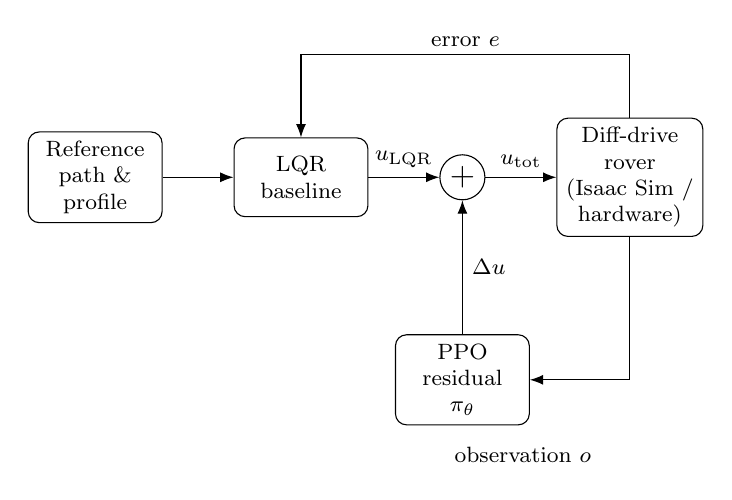
\begin{tikzpicture}[
  font=\footnotesize,
  block/.style={draw, rounded corners, minimum width=1.7cm, minimum height=1.0cm, align=center},
  sum/.style={draw, circle, inner sep=1.5pt},
  >=Latex
]
% top row: path -> LQR -> (+) -> rover
\node[block] (path) {Reference\\path \&\\profile};
\node[block, right=0.9cm of path] (lqr) {LQR\\baseline};
\node[sum, right=0.9cm of lqr] (sum) {\large$+$};
\node[block, right=0.9cm of sum] (rover) {Diff-drive\\rover\\(Isaac Sim /\\hardware)};
% PPO residual well below the summing junction
\node[block, below=1.7cm of sum] (ppo) {PPO\\residual\\$\pi_\theta$};
% forward signal path
\draw[->] (path) -- (lqr);
\draw[->] (lqr) -- node[above]{$u_{\text{LQR}}$} (sum);
\draw[->] (sum) -- node[above]{$u_{\text{tot}}$} (rover);
% residual feeds straight up into the sum (clean vertical line)
\draw[->] (ppo) -- node[right]{$\Delta u$} (sum);
% observation feedback: down from rover, then left into the RIGHT side of PPO
\coordinate (obs) at (rover.south |- ppo.east);
\draw[->] (rover.south) -- (obs) -- (ppo.east);
\node[anchor=north east] at ($(ppo.south east)+(0.9cm,-0.15cm)$) {observation $o$};
% error feedback: up from rover, across the top, down into LQR
\draw[->] (rover.north) -- ++(0,0.8) -| (lqr.north);
\node[above, yshift=3pt] at ($(rover.north)!0.5!(lqr.north)+(0,0.8)$) {error $e$};
\end{tikzpicture}%
}
\caption{Hybrid LQR{+}PPO residual control architecture. The LQR baseline guarantees stable, interpretable tracking from path-frame errors only (slip-blind by design); the bounded PPO residual $\Delta u$, which observes per-wheel slip and sinkage, corrects for soft-soil effects the linear model cannot capture. Pure-LQR uses only the upper path; pure-PPO replaces the baseline with a direct policy command.}
\label{fig:architecture}
\end{figure}

\subsection{Vehicle Model}
We employ a differential-drive Leo Rover controlled by velocity inputs $u = [v, \omega]^T$, where $v$ is the forward velocity and $\omega$ is the angular velocity. The platform is equipped with an IMU for orientation/acceleration, wheel encoders for velocity estimation, and an XVisio SeerSense DS80 stereo camera for forward terrain perception. The kinematic model follows standard unicycle/differential-drive dynamics:
\begin{align}
\dot{x} &= v \cos(\theta), &
\dot{y} &= v \sin(\theta), &
\dot{\theta} &= \omega,
\end{align}
where $(x, y)$ is the position and $\theta$ is the heading. The commanded body velocity is mapped to left/right wheel angular velocities by the differential-drive relation $\dot{\phi}_{L,R} = (v \mp \omega L)/(2r)$, with wheel base $L = 0.34$~m and wheel radius $r = 0.0625$~m. Velocity commands are limited to the Leo Rover hardware envelope, $|v| \le 0.4$~m/s and $|\omega| \le 1.047$~rad/s ($\approx 60^\circ$/s). On deformable terrain, slip and sinkage introduce discrepancies between commanded and actual velocities, which we address through the hybrid control framework.

\subsection{LQR Baseline Controller}
The LQR controller stabilizes tracking by regulating a path-frame error state to zero. We use the linearized unicycle error model with state
\begin{equation}
\mathbf{e} = [e_{\text{lat}},\; e_{\theta},\; e_{v}]^T,
\end{equation}
where $e_{\text{lat}}$ is the signed lateral (cross-track) offset, $e_{\theta}$ is the heading error, and $e_{v} = v - v_{\text{ref}}$ is the velocity error relative to the trajectory-profile reference speed $v_{\text{ref}}$. The linearized error dynamics are $\dot{\mathbf{e}} = A\mathbf{e} + B\Delta\mathbf{u}$ with
\begin{equation}
A = \begin{bmatrix} 0 & v_{\text{ref}} & 0 \\ 0 & 0 & 0 \\ 0 & 0 & -1 \end{bmatrix},\quad
B = \begin{bmatrix} 0 & 0 \\ 0 & 1 \\ 1 & 0 \end{bmatrix},
\end{equation}
so that the heading channel actuates lateral error through the forward speed and the velocity channel directly regulates $e_v$. The controller minimizes the quadratic cost
\begin{equation}
J = \int_0^\infty \left(\mathbf{e}^T Q \mathbf{e} + \Delta\mathbf{u}^T R \Delta\mathbf{u}\right) dt,
\end{equation}
with $Q = \mathrm{diag}(10,\,6,\,0.5)$ and $R = \mathrm{diag}(0.5,\,0.8)$, yielding the optimal gain $K = R^{-1}B^T P$, where $P$ solves the continuous-time algebraic Riccati equation. The baseline command is
\begin{equation}
\mathbf{u}_{\text{LQR}} = [v_{\text{ref}},\, \omega_{\text{ref}}]^T - K\mathbf{e}.
\end{equation}
Because $A$ depends on $v_{\text{ref}}$, the gain $K(v_{\text{ref}})$ is gain-scheduled: it is precomputed on a fine grid of reference speeds and interpolated online. The controller is evaluated in a GPU-vectorized implementation so all parallel environments share the identical baseline. We emphasize a deliberate design choice: the LQR observes only path-frame kinematic errors. It receives \emph{no} slip or sinkage information, so it represents the best a well-tuned linear tracking law can do without a soil model, which is exactly the capability gap the residual is meant to fill.

\subsection{PPO Residual Policy}
The PPO agent outputs a bounded corrective command $\Delta\mathbf{u}$ that is added to the baseline,
\begin{equation}
\mathbf{u}_{\text{tot}} = \mathbf{u}_{\text{LQR}} + \Delta\mathbf{u}, \qquad
\Delta\mathbf{u} = \alpha \left[\Delta v_{\max} a_1,\; \Delta\omega_{\max} a_2\right]^T,
\end{equation}
where $\mathbf{a}\in[-1,1]^2$ is the raw policy action, $\Delta v_{\max}=0.15$~m/s and $\Delta\omega_{\max}=0.30$~rad/s are the base residual bounds, and $\alpha=0.5$ is a fixed residual-authority scale. The effective residual envelope is therefore $|\Delta v| \le 0.075$~m/s and $|\Delta\omega| \le 0.15$~rad/s ($19\%$ of $v_{\max}$ and $14\%$ of $\omega_{\max}$), keeping the learned correction strictly subordinate to the stabilizing baseline. The authority scale is a training-time constant and must match at evaluation; all results in this paper use $\alpha=0.5$. In the pure-PPO ablation, the policy instead emits the full command $[v,\omega]$ directly. The combined command is clipped to the hardware envelope before the differential-drive mapping.

\vspace{1mm}
\noindent\textbf{Observation.} The policy $\pi_\theta$ receives a proprioceptive-plus-terrain observation:
\begin{align}
\mathbf{o} = \big[ &\, e_{\text{lat}},\, e_{\theta},\, v_{\text{fwd}},\, v_{\text{lat}},\, \Delta x^{b}_{\text{wp}},\, \Delta y^{b}_{\text{wp}}, \nonumber\\
& \underbrace{v_{\text{base}},\, \omega_{\text{base}}}_{\text{hybrid only}},\, g^{b}_{x},\, g^{b}_{y},\, g^{b}_{z},\, \mathbf{s}_{\text{terrain}},\, \underbrace{\mathbf{s}_{\text{slip}},\, \mathbf{z}_{\text{sink}}}_{\text{soil model on}} \big],
\end{align}
where $v_{\text{fwd}}, v_{\text{lat}}$ are body-frame velocities; $(\Delta x^{b}_{\text{wp}}, \Delta y^{b}_{\text{wp}})$ is the next-waypoint vector in the body frame; $(v_{\text{base}},\omega_{\text{base}})$ is the LQR baseline command (provided only to the hybrid policy so the residual is aware of the baseline it is correcting); $\mathbf{g}^{b}$ is the gravity vector projected into the body frame, encoding the local terrain tilt under the chassis; $\mathbf{s}_{\text{terrain}}\in\mathbb{R}^{6}$ contains forward terrain-slope features (longitudinal and cross-path slope) for near ($0$--$0.7$~m), mid ($0.7$--$1.2$~m), and far ($1.2$--$2.0$~m) zones from a forward, downward-facing height scanner that emulates the stereo camera's terrain lookahead; and, when the deformable-soil layer is active, $\mathbf{s}_{\text{slip}}\in\mathbb{R}^{4}$ and $\mathbf{z}_{\text{sink}}\in\mathbb{R}^{4}$ are the per-wheel longitudinal slip ratios and sinkage states of Section~\ref{sec:soil}. This yields a $15$-dimensional observation for pure PPO and $17$ for the hybrid on rigid terrain, growing to $23$ and $25$ respectively with the soil model. The slip/sinkage block is the decisive input: it gives the residual direct, per-wheel awareness of traction loss that neither the LQR nor any purely kinematic observation can provide.

\vspace{1mm}
\noindent\textbf{Reward.} The reward uses dense shaping to encourage accurate path adherence while limiting excessive control effort and rewarding progress:
\begin{align}
r_t = &-w_{\text{cte}}\, e_{\text{lat}}^2 \;-\; w_{\theta}\, e_{\theta}^2 \;+\; w_{v}\, \rho(e_{\text{lat}})\, v_{\text{fwd}}^{+} \nonumber\\
& -\; w_{\text{sm}}\big(|\Delta v_t| + |\Delta\omega_t|\big) \;+\; w_{p}\, \Delta p_t \nonumber\\
& +\; R_{\text{succ}}\,\mathbb{1}[\text{goal}] \;-\; R_{\text{fail}}\,\mathbb{1}[\text{fail}],
\end{align}
where $\rho(e_{\text{lat}}) = \max\!\big(0,\,1 - |e_{\text{lat}}|/c\big)$ with $c=0.5$~m ramps the forward-speed reward down as the rover leaves the path, $v_{\text{fwd}}^{+}=\max(0,v_{\text{fwd}})$, and $\Delta p_t$ is the increment in along-path progress with $w_p = 150$, making progress the dominant dense term. \verify{remaining dense weights $w_{\text{cte}}, w_{\theta}, w_{v}, w_{\text{sm}}$ and terminal magnitudes $R_{\text{succ}}, R_{\text{fail}}$ against config.py}

For the hybrid policy, three residual-specific terms are added. First, a residual-effort penalty $-w_{\text{eff}}\lVert\Delta\mathbf{u}_{\text{norm}}\rVert^2$ discourages overriding the stable baseline unnecessarily. This term proved sharply double-edged: with an early setting $w_{\text{eff}}=0.5$ the residual collapsed to zero and training stalled near the pure-LQR level; the final value is $w_{\text{eff}}=0.01$. Second, to give the residual \emph{positive} credit rather than only penalties, a baseline-relative credit term
\begin{equation}
r_{\text{credit}} = w_{c}\,\big(\hat{c}_{\text{LQR}} - \hat{c}_{\text{tot}}\big), \qquad w_c = 15,
\end{equation}
rewards the one-step-ahead predicted cross-track improvement of the combined command over what the baseline alone would have produced, where $\hat{c}$ is a kinematic one-step rollout of the respective command. This term is what allows a small residual to survive the effort penalty when, and only when, it demonstrably improves tracking. Third, on deformable soil we introduce a slip-gated exemption on the velocity channel of the effort penalty: the $\Delta v$ penalty is scaled by $1-\lambda(\bar{s})$, where $\lambda$ ramps linearly from $0$ at mean wheel slip $\bar{s}=0.35$ (normal sand rolling) to $1$ at $\bar{s}=0.70$ (dig-in), so speed corrections become free exactly when escaping entrapment requires them, while the steering channel remains regularized. Episode failure conditions are: cross-track error exceeding $2$~m, stagnation (no progress for a fixed window), flipping, leaving the path-extent bounding box, or timeout. Slip is recorded as an evaluation metric rather than a reward term.

\vspace{1mm}
\noindent\textbf{Network architecture and optimization stability.} The actor and critic are separate multilayer perceptrons, each with two hidden layers of $256$ units and ReLU activations, preceded by running observation normalization. The policy is a diagonal Gaussian with a state-independent, learned standard deviation. We found that at 4{,}096-environment scale, the noise standard deviation is a critical failure axis: in one training run the entropy bonus drove $\sigma$ into a positive-feedback runaway (larger $\sigma$ yields more entropy reward, which yields larger $\sigma$) that terminated in numerical overflow, while the policy's rollouts degenerated into baseline-plus-uniform-noise. Lowering the entropy coefficient alone produced the opposite failure ($\sigma$ frozen at its initialization, no exploration). The robust fix is structural: after every PPO update, $\sigma$ is clamped to $[0.05, 0.6]$. Within this corridor the trained policy self-regulates ($\sigma \approx 0.06$--$0.08$ late in training, above the floor, indicating exploration retained value). The entropy coefficient is $0.001$. Optimization uses a KL-adaptive learning-rate schedule (target KL $0.02$, base learning rate $1.5\times10^{-4}$ \verify{lr and target KL against train cfg}), clip range $0.2$, $5$ epochs per update, discount $\gamma=0.99$, and GAE $\lambda=0.95$. We selected this compact architecture deliberately: the observation is low-dimensional and the action two-dimensional, so a $2\times256$ MLP provides ample capacity without slowing the massively parallel rollouts; a recurrent variant \cite{alcayaga2025lstm} is a natural extension, but the memoryless policy with explicit slip observation already captures the required signal.

\subsection{Deformable-Terrain Model: Terramechanics-Lite}
\label{sec:soil}
A key claim of this paper is that the value of residual learning is gated by contact fidelity, so the fidelity mechanism itself must be stated precisely. We are explicit about what is and is not simulated: \emph{the sand is not simulated as a granular material}. Particle-based approaches (DEM/PBD/MPM) that resolve individual grains cost more per step for one rover than our entire 4{,}096-rover fleet \cite{orsula2025sim2dust}, and PhysX collision meshes are immutable after cooking, so true runtime terrain deformation is unavailable in this simulator class. Instead, the ground remains a rigid procedural mesh, and at every control step we compute, per wheel, the \emph{forces that soft soil would exert} and apply their resultant as an external wrench on the chassis. Injecting semi-empirical terramechanics forces into an otherwise rigid multibody simulation follows the soil-contact-model approach established for planetary rover simulators by Krenn and Hirzinger \cite{krenn2009scm}; our layer is a deliberately reduced, GPU-vectorized form of that lineage \cite{bekker1969introduction, wong2008theory, ishigami2007terramechanics, taheri2015technical}, retaining the three phenomena that rigid Coulomb contact structurally cannot express.

\vspace{1mm}
\noindent\textbf{Per-wheel slip.} For wheel $i$ with commanded rim speed $r\dot{\phi}_i$ and body-frame hub velocity $v_{\text{hub},i}$ (computed from the chassis twist and the wheel's mounting offsets), the longitudinal slip ratio is
\begin{equation}
s_i = \mathrm{clip}\!\left(\frac{r\dot{\phi}_i - v_{\text{hub},i}}{\max(|r\dot{\phi}_i|,\, v_\epsilon)},\, -1,\, 1\right), \quad v_\epsilon = 0.05~\text{m/s},
\end{equation}
zeroed below a $0.02$~m/s rim-speed deadband. This is the standard drive-slip definition: $s_i \rightarrow 1$ means the wheel spins without advancing.

\vspace{1mm}
\noindent\textbf{Mechanism 1: sinkage with dig-in memory.} Each wheel carries a normalized sinkage state $z_i \in [0,1]$ with first-order dynamics
\begin{equation}
\dot{z}_i = k_{\text{dig}}\, |s_i|\, \zeta_i \;-\; k_{\text{rec}}\, (1 - |s_i|)\,\mathbb{1}[\text{moving}],
\end{equation}
so slipping \emph{digs} the wheel in (faster in softer soil $\zeta_i$) and clean rolling gradually climbs back out. Sinkage feeds a motion-resistance force
\begin{equation}
F_{\text{roll},i} = -\big(c_{\text{rr}} + c_{z} z_i\big)\, \zeta_i\, N\, \tanh(v_{\text{hub},i}/v_0),
\end{equation}
with $v_0 = 0.05$~m/s. This gives sand the \emph{memory} rigid friction lacks: a few seconds of wheelspin raises per-wheel drag from about $-0.6$~N (clean rolling) to about $-9$~N (fully dug in), and the only exit is patient low-slip rolling.

\vspace{1mm}
\noindent\textbf{Mechanism 2: slip-thrust decay.} Coulomb friction is flat past its static peak, so on rigid ground a spinning wheel still delivers full tractive force and ``more throttle'' is never punished. Real sand's thrust curve peaks near $20$--$30\%$ slip and \emph{decays} beyond it as the wheel excavates its own support \cite{wong2008theory, ishigami2007terramechanics}. We model the post-peak deficit as
\begin{equation}
F_{\text{slip},i} = -c_{s}\, \zeta_i\, N\, \max(0,\, |s_i| - s_{\text{pk}})\,\mathrm{sgn}(r\dot{\phi}_i),
\end{equation}
with peak slip $s_{\text{pk}} = 0.25$. This single term makes throttle-into-slip (precisely the failure response of a slip-blind linear controller) physically counterproductive.

\vspace{1mm}
\noindent\textbf{Mechanism 3: saturating lateral shear.} Sand resists side-slip plastically rather than rigidly:
\begin{equation}
F_{\text{lat},i} = -c_{\ell}\, \zeta_i\, N\, \tanh(v_{\text{lat},i}/v_1), \quad v_1 = 0.10~\text{m/s},
\end{equation}
producing downhill creep on tilted soil and widened arcs in turns.

\vspace{1mm}
\noindent\textbf{Soil heterogeneity.} All three mechanisms scale with a static soil-softness field $\zeta(x,y) \in [0,1]$: seeded value noise on a $2$~m cell grid, twice smoothed, min--max normalized, and sharpened with exponent $1.5$, yielding continuous firm-to-soft variation with roughly $28\%$ of the world effectively sandy. Because $\zeta$ is a pure function of the global seed, every controller in a paired evaluation traverses the byte-identical soil field; heterogeneous traction is part of the matched conditions, not noise. Per-wheel loads use the static approximation $N = m g / 4 \approx 13.5$~N.

\vspace{1mm}
\noindent\textbf{Application and cost.} The four wheels' forces and their yaw moments (from the mounting lever arms) are summed into a single body-frame wrench applied to the chassis link each $0.2$~s control step. The entire model is approximately twenty tensor operations on a $[4096 \times 4]$ grid, negligible against physics stepping, and every term opposes its conjugate velocity, so the layer is dissipative by construction and cannot inject energy. Table~\ref{tab:soil_coeffs} lists the coefficients; all are exposed as environment parameters for later calibration.

\begin{table}[t]
\centering
\caption{Terramechanics-Lite Coefficients}
\label{tab:soil_coeffs}
{\footnotesize
\setlength{\tabcolsep}{4pt}
\begin{tabular}{@{}llll@{}}
\toprule
\textbf{Symbol} & \textbf{Meaning} & \textbf{Value} & \textbf{Units} \\
\midrule
$c_{\text{rr}}$ & baseline rolling resistance & $0.04$ & -- \\
$c_{z}$ & sinkage drag gain & $0.30$ & -- \\
$s_{\text{pk}}$ & peak-thrust slip ratio & $0.25$ & -- \\
$c_{s}$ & post-peak thrust-decay gain & $0.50$ & -- \\
$c_{\ell}$ & lateral shear gain & $0.35$ & -- \\
$k_{\text{dig}}$ & sinkage growth rate & $0.50$ & s$^{-1}$ \\
$k_{\text{rec}}$ & sinkage recovery rate & $0.25$ & s$^{-1}$ \\
-- & zone-sharpening exponent & $1.5$ & -- \\
$N$ & static per-wheel load & $13.5$ & N \\
\bottomrule
\end{tabular}
}
\end{table}

\vspace{1mm}
\noindent\textbf{Scope of the realism claim.} The model reproduces the \emph{phenomenology} of sand (progressive dig-in, thrust loss under aggressive slip, plastic lateral resistance, and spatially heterogeneous traction) with coefficients chosen for plausibility, not calibrated to a specific regolith simulant. It omits inter-wheel load transfer, persistent ruts (the terrain mesh does not deform), and the full Bekker pressure--sinkage integral. Two observations support its face validity beyond construction: first, verified force magnitudes remain within the physically sensible envelope (worst-case total soil drag of $\approx\!22$~N against $\approx\!64$~N of available traction, so the rover is impeded, never glued); second, the model produced emergent behaviors that were never programmed, including flat-ground bog-downs at cruise speed (maximum commanded speed produces maximum slip and hence dig-in, inverting the usual difficulty ordering; Section~\ref{sec:sandresults}) and gradual entrapment failures near $70\%$ progress replacing geometric crashes. Calibrating the coefficients against measured slip and drawbar pull from the physical sand pit is an explicit step of the hardware phase (Section~\ref{sec:realworld}).

\subsection{Simulation Environment}
We build the training environment in NVIDIA Isaac Sim 4.5 with the Isaac Lab framework \cite{mittal2023orbit, makoviychuk2021isaac}. Isaac Lab provides GPU-resident, vectorized physics so that thousands of rover instances advance in parallel; we train with $4096$ parallel environments on a single RTX 4090 GPU. Key environment settings:
\begin{itemize}
\item \textbf{Physics and control rate:} physics step $1/50$~s with a decimation of $10$, giving a $0.2$~s control step. Wheels are velocity-controlled. \verify{gravity setting used in the reported runs (Mars $3.71$ vs.\ Earth $9.81$~m/s$^2$); the soil-load constant assumes Earth gravity}
\item \textbf{Episode configuration:} up to $400$~s ($2000$ control steps) or until the goal is reached, the rover flips, leaves the path-extent bounds, stagnates, or exceeds the $2$~m cross-track limit. For cap-sensitivity analyses the episode limit is extensible (Section~\ref{sec:sandresults}).
\item \textbf{Terrain bank:} procedurally generated Gaussian-hill height fields on a $0.025$~m grid, organized as $6$ difficulty rows $\times$ $2$ variants of $12$~m patches with row-exact intensities $\{0, 20, 40, 60, 80, 100\}\%$ (peak amplitude $1.5$~m at $100\%$). A cosine edge taper ($1.5$~m) blends each patch into its border, eliminating artificial walls at patch boundaries. The modest bank size is set by the PhysX collision-mesh budget at this resolution; per-episode patch assignment and per-patch seeding provide variety.
\item \textbf{Domain randomization:} per-episode, per-wheel randomization of wheel--terrain friction over $\mu \in [0.47, 2.0]$, and per-episode reassignment of each rover to a randomly drawn terrain patch and a fresh reference path.
\item \textbf{Deformable-soil layer:} the terramechanics-lite model of Section~\ref{sec:soil}, active in all Phase-2 (sand) experiments; the identical pipeline with the layer disabled constitutes the rigid-contact control condition.
\item \textbf{Forward terrain sensing:} a downward ray-caster ahead of the chassis emulates the stereo camera, producing the near/mid/far slope features used in the observation.
\end{itemize}
Figure~\ref{fig:sim_screenshot} shows a representative view of the parallel training environment.

\begin{figure}[t]
\centering
\fbox{\begin{minipage}[c][3.2cm][c]{0.92\columnwidth}\centering\itshape [PLACEHOLDER: screenshot of the Isaac Sim training environment, showing rovers on procedurally generated Mars-like terrain with reference paths overlaid.]\end{minipage}}
\caption{Parallel rover training environment in NVIDIA Isaac Sim / Isaac Lab.}
\label{fig:sim_screenshot}
\end{figure}

\begin{figure}[t]
\centering
\fbox{\begin{minipage}[c][3.2cm][c]{0.92\columnwidth}\centering\itshape [PLACEHOLDER: two-panel figure. Left: soil-softness field $\zeta(x,y)$ over the world (heat map, 2~m cells, seed-locked). Right: schematic of the three wheel-level soil forces (sinkage drag, slip-thrust decay, lateral shear) acting on one wheel.]\end{minipage}}
\caption{Terramechanics-lite soil layer: seeded heterogeneous softness field and the three dissipative wheel-level force mechanisms.}
\label{fig:soil_model}
\end{figure}

\subsection{Training Protocol}
\label{sec:training}
Rather than a small fixed path library, each episode draws a reference path from a bank of $500$ procedurally generated random curved paths (seeded for reproducibility), with per-segment curvature between $25^\circ$ and $120^\circ$ and a total path length of $10$~m. This continuous variety, rather than a handful of hand-designed shapes, drives generalization during training.

\vspace{1mm}
\noindent\textbf{Terrain curriculum: a negative result.} We initially coupled training to an automatic domain-randomization (ADR) curriculum that ramps the terrain-difficulty ceiling with competence, following \cite{rudin2022learning}. For the \emph{hybrid} policy this proved counterproductive: because the LQR baseline already prevents catastrophic failure on hard terrain, the ramp merely starved the residual of the very episodes (steep, low-traction) where it has something to learn, and early-training statistics were dominated by terrain the baseline alone solves. All reported hybrid runs therefore sample terrain difficulty \emph{uniformly over the full range from the first step}, which trained stably. The ramped curriculum is retained only for the unprotected pure-PPO configuration, where early exposure to hard terrain does cause divergence. We highlight this as a practical guideline: a residual policy inherits the baseline's safety, and with it, the freedom to train on the hardest terrain immediately.

\vspace{1mm}
\noindent\textbf{Optimization scale.} The policy is optimized with PPO \cite{schulman2017proximal} using a GPU-vectorized on-policy runner. Each update collects $32$ steps per environment ($\approx 131{,}000$ transitions per iteration across $4096$ environments). The principal sand-trained policy reported here ran $25{,}400$ updates ($\approx 3.3\times10^{9}$ environment steps; $6.4$ million completed episodes) in $2.2$ days at a sustained $\approx\!24{,}000$ steps/s on the single training GPU. Deterministic-policy evaluation success on held-out random paths climbed from $62\%$ (LQR-equivalent early plateau) to $80$--$81\%$ at convergence. Episodic reward, length, residual-channel magnitudes, and noise std are logged throughout.

\subsection{Deployment Strategy}
To bridge the sim-to-real gap, we rely on (i) domain randomization over friction, terrain, and heterogeneous soil zones; (ii) the LQR baseline, which supplies safe, interpretable behavior during early deployment and bounds the effect of an imperfect residual; (iii) planned calibration of the soil-layer coefficients against physical slip/drawbar measurements from the sand pit; and (iv) safety mechanisms, including emergency-stop conditions on heading error ($>90^\circ$) and wheel-current limits, inspired by NASA ACE clearance evaluation \cite{nasaACE}. We do not use a separate teacher-student distillation stage; the hybrid structure itself provides the stable ``teacher-like'' behavior that residual learning refines.

\section{Experiments}
\subsection{Experimental Design}
\subsubsection{Goals and Research Questions}
The primary objective is to evaluate whether the hybrid LQR{+}PPO residual controller achieves superior path-following on dynamic terrain compared to its constituent baselines, under conditions that isolate the controller as the only variable, and to identify \emph{which environmental conditions} create the residual's advantage. Key research questions:
\begin{itemize}
\item \textbf{RQ1:} Does the hybrid approach achieve lower cross-track error than pure LQR and pure PPO, and does the advantage depend on contact fidelity (rigid vs.\ deformable soil)?
\item \textbf{RQ2:} Does the hybrid method converge faster (improved sample efficiency) than pure PPO?
\item \textbf{RQ3:} Is the hybrid controller more robust to terrain variation; in particular, does its performance degrade least as a function of realized wheel slip, terrain difficulty, and slope?
\item \textbf{RQ4:} How does performance vary across discrete path geometries (zig-zag, curved, closed polygon)?
\item \textbf{RQ5:} Does the hybrid controller \emph{complete} more paths, i.e.\ achieve a higher task-success rate, than pure LQR and pure PPO?
\end{itemize}

\subsubsection{Compared Methods}
We compare three controllers, which share the identical vehicle model, observation pipeline, and evaluation conditions, differing only in the control policy:
\begin{enumerate}
\item \textbf{LQR-only:} the deterministic baseline of Section~III-B with fixed, gain-scheduled feedback (slip-blind by design).
\item \textbf{PPO-only:} an end-to-end policy that outputs $[v,\omega]$ directly, with no LQR baseline.
\item \textbf{LQR{+}PPO (Hybrid):} our proposed method, where PPO outputs a bounded residual added to the LQR baseline.
\end{enumerate}
\noindent\emph{Status note.} Under the deformable-soil configuration, the end-to-end PPO baseline has not yet produced a competent policy at a matched training budget in this pipeline (training remained far below baseline competence); its entries in the sand-condition tables are marked pending and its full retraining with the soil observation is in progress. This is itself consistent with the sample-inefficiency and instability findings that motivate the hybrid design \cite{blum2020ppmc, johannink2019residual}, but we refrain from quantitative PPO-column claims until the retrained baseline is complete.

\subsection{Simulation Experiments}
\subsubsection{Matched-Condition (Scenario-Locked) Comparison}
A central design choice is that controllers are evaluated on \emph{exactly the same} episodes. For the paired suites, a scenario file pre-draws, for each of $90{,}000$ episode slots: the reference path, the terrain patch assignment, and the start pose; the seeded soil field is identical by construction, and friction is held fixed within a suite (and swept across suites) because per-episode friction draws cannot be reproduced across separately launched runs. Each controller then consumes the identical scenario list, so any difference in outcome is attributable to the controller alone, and paired statistics (paired $t$ on per-scenario cross-track error, McNemar on per-scenario success outcomes, Cohen's $d_z$, Bonferroni-corrected) are valid. Success is \emph{progress-gated}: an episode counts as successful only if the rover reaches the final waypoint within tolerance \emph{and} has traversed at least $90\%$ of the path. The gate matters: for closed polygon paths the goal coincides with the start, and without the gate a stationary controller scores $100\%$ instantly, an artifact that inflated early evaluations and that we flag for practitioners.

\subsubsection{Evaluation Protocol}
Each controller is evaluated along two complementary dimensions.

\noindent\textbf{Dimension 1 -- Path geometry (discrete, paired).} Nine fixed test paths spanning three categories (three zig-zag, three curved, three closed-polygon variants), instantiated across terrain difficulties and repeated to $90{,}000$ matched episodes per controller.

\noindent\textbf{Dimension 2 -- Randomized terrain (training-distribution, logged).} Random curved paths with per-episode random terrain level, patch, and per-wheel friction, evaluated deterministically at scale ($n \approx 12{,}000$--$14{,}000$ episodes per controller). Because per-episode terrain level, realized slip, local slope, and friction are logged, performance can be conditioned post hoc on each of these variables. All evaluations use deterministic policy execution.

\subsubsection{Performance Metrics}
For each episode we record cross-track error statistics, realized per-wheel slip (rim-vs-hub when the soil layer is active; commanded-vs-actual as the rigid-terrain proxy), local slope, terrain level, friction, path progress, episode length, and outcome. Per-episode summaries:
\begin{itemize}
\item \textbf{Mean cross-track error (MCTE):} $\frac{1}{T}\sum_t |e_{\text{lat}}(t)|$, the primary tracking metric.
\item \textbf{Success rate:} proportion of episodes reaching the final waypoint within tolerance with the $90\%$ progress gate.
\item \textbf{Slip statistics:} mean and maximum realized slip.
\item \textbf{Failure diagnostics:} progress at failure, timeout vs.\ early-termination fractions, and a ``parked'' indicator (timeout with $<10\%$ progress).
\end{itemize}

\subsubsection{Rigid-Contact Control Condition}
\label{sec:rigidresults}
We first report the Phase-1 result that motivated the soil layer. On the rigid-contact version of the environment (identical terrain, friction randomization, paths; no soil forces; observation without the slip/sinkage block), the best hybrid policy was compared to LQR over $90{,}000$ paired scenarios at high friction: success $45.7\%$ vs.\ $43.5\%$ under gate-corrected scoring ($+2.2$ points; McNemar $\chi^2 = 294.7$, discordant $6779/4921$, $p < 10^{-4}$), and MCTE $0.202$ vs.\ $0.206$~m ($\Delta \approx -4$~mm; paired $t = -15.7$, $d_z = 0.053$, $p < 10^{-4}$). (Test statistics are computed on the archived paired suite, which predates the progress gate; its polygon auto-completions inflate absolute success identically for both controllers and leave the paired comparisons intact, so success percentages are quoted from the gate-corrected re-scoring.) The gain, moreover, was localized: it concentrated in agility-limited cells, most strikingly a roughly $5\times$ success ratio ($\approx\!49\%$ vs.\ $\approx\!10\%$) on flat sharp-zigzag scenarios where LQR enters a limit cycle around hairpins, while across most of the terrain distribution the two controllers were statistically indistinguishable. A low-friction paired suite showed no success advantage at all ($33.8\%$ vs.\ $34.5\%$) and only a small tracking effect ($d_z \approx 0.08$). Extensive reward-shaping variants on the rigid world failed to widen this gap and several regressed, which we interpret structurally: \emph{on rigid Coulomb contact, a well-tuned LQR is already near the performance ceiling, and no reward reshaping can conjure headroom the physics does not provide.} This negative result directly motivated Section~\ref{sec:soil}.

\subsubsection{Deformable-Soil Results}
\label{sec:sandresults}
All Phase-2 results use the identical pipeline with the terramechanics-lite layer enabled and the slip/sinkage observation block active; the LQR baseline is unchanged (and remains slip-blind).

\vspace{1mm}
\noindent\textbf{Randomized-terrain suite (primary).} Table~\ref{tab:sand_levels} reports the same-harness deterministic evaluation on random paths over the full terrain-difficulty range with per-episode random friction. The hybrid improves \emph{both} metrics at \emph{every} terrain level: overall success $83.4\%$ vs.\ $79.3\%$ ($+4.1$ points) and MCTE $0.073$~m vs.\ $0.137$~m ($-47\%$). The largest success gains sit at the distribution's extremes (flat: $+7.3$; maximum difficulty: $+9.4$), and the tracking gain is largest precisely on flat sand ($0.037$ vs.\ $0.131$~m, $-72\%$), where the slip-blind baseline cruises at maximum speed and pays maximum slip. Note the difficulty inversion in the LQR column: level $20$ outperforms level $0$ ($97.8\%$ vs.\ $87.6\%$), because gentle hills force lower commanded speeds that incidentally manage slip. On deformable soil, \emph{soil interaction, not geometry, is the difficulty axis}, and flat ground is where a slip-blind controller is most aggressive and therefore most vulnerable. The hybrid, which observes slip directly, largely removes this vulnerability. ``Parked'' outcomes (timeout with $<\!10\%$ progress) drop from $0.03\%$ to $0.01\%$; both controllers' residual failures are dominated by mid-path entrapment (median failure progress $\approx\!68$--$70\%$), not by never starting.

\begin{table}[t]
\centering
\caption{Deformable Soil, Randomized-Terrain Suite: Success and MCTE by Terrain Level (Deterministic Policies, Per-Episode Random Friction; $n_{\text{Hybrid}}=14{,}013$, $n_{\text{LQR}}=12{,}224$)}
\label{tab:sand_levels}
\resizebox{\columnwidth}{!}{%
\begin{tabular}{@{}lcccccc@{}}
\toprule
& \multicolumn{2}{c}{\textbf{LQR}} & \multicolumn{2}{c}{\textbf{Hybrid}} & \multicolumn{2}{c}{\textbf{$\Delta$ (H$-$L)}} \\
\cmidrule(lr){2-3}\cmidrule(lr){4-5}\cmidrule(l){6-7}
\textbf{Level} & Succ.\ (\%) & MCTE (m) & Succ.\ (\%) & MCTE (m) & Succ. & MCTE \\
\midrule
0 (flat) & 87.6 & 0.131 & 94.9 & 0.037 & $+7.3$ & $-0.094$ \\
20 & 97.8 & 0.055 & 98.1 & 0.040 & $+0.4$ & $-0.015$ \\
40 & 82.7 & 0.163 & 85.6 & 0.079 & $+2.9$ & $-0.084$ \\
60 & 79.1 & 0.125 & 81.7 & 0.072 & $+2.7$ & $-0.053$ \\
80 & 56.1 & 0.173 & 57.1 & 0.130 & $+1.0$ & $-0.043$ \\
100 & 73.1 & 0.180 & 82.5 & 0.080 & $+9.4$ & $-0.100$ \\
\midrule
\textbf{Overall} & \textbf{79.3} & \textbf{0.137} & \textbf{83.4} & \textbf{0.073} & $\mathbf{+4.1}$ & $\mathbf{-0.064}$ \\
\bottomrule
\end{tabular}%
}
\\[2pt]
{\footnotesize PPO-only column pending (see Compared Methods status note).}
\end{table}

\vspace{1mm}
\noindent\textbf{Slip-conditioned robustness (RQ3).} Table~\ref{tab:slip_tertiles} conditions the same suite on realized mean wheel slip (tertile bounds computed on the pooled distribution, $s < 0.380$ / $0.380$--$0.419$ / $\ge 0.419$). The two controllers are nearly identical in benign-slip episodes; the gap opens monotonically with slip and becomes decisive in the top tertile: success $62.1\%$ vs.\ $50.2\%$ ($+11.9$ points) and MCTE $0.129$ vs.\ $0.318$~m ($-59\%$). Conditioning on local slope shows the same pattern compressed (high-slope tertile: $65.4\%$ vs.\ $63.6\%$ success, $0.118$ vs.\ $0.156$~m MCTE), and slope conditioning also reproduces the inversion (for LQR, \emph{low}-slope episodes carry the worst tracking error, $0.145$~m, again because flat terrain invites full-speed slip). Slip, not slope, is the variable that separates the controllers; that is exactly the signature a slip-aware residual should produce, and the flattest performance-vs-slip curve answers RQ3 in the hybrid's favor.

\begin{table}[t]
\centering
\caption{Deformable Soil: Performance Conditioned on Realized Mean Wheel Slip (Pooled Tertile Bounds $0.380$ / $0.419$)}
\label{tab:slip_tertiles}
{\footnotesize
\setlength{\tabcolsep}{4pt}
\begin{tabular}{@{}lcccc@{}}
\toprule
& \multicolumn{2}{c}{\textbf{LQR}} & \multicolumn{2}{c}{\textbf{Hybrid}} \\
\cmidrule(lr){2-3}\cmidrule(l){4-5}
\textbf{Slip tertile} & Succ.\ (\%) & MCTE (m) & Succ.\ (\%) & MCTE (m) \\
\midrule
Low & 97.4 & 0.041 & 98.3 & 0.037 \\
Middle & 88.6 & 0.060 & 92.0 & 0.048 \\
High & 50.2 & 0.318 & 62.1 & 0.129 \\
\bottomrule
\end{tabular}
}
\end{table}

\vspace{1mm}
\noindent\textbf{Paired discrete-geometry suite (RQ4).} On the $90{,}000$-episode scenario-locked suite over the nine fixed geometries, the hybrid's tracking advantage is universal: MCTE $0.4175$ vs.\ $0.4721$~m ($\Delta = -5.5$~cm; paired $t = -90.8$, $p < 10^{-4}$, $d_z = 0.30$), and the hybrid has lower MCTE in \emph{every} geometry and slope cell of the suite: $-3.5$~cm on curved, $-7.2$~cm on zig-zag, $-5.7$~cm on polygon paths, and up to $-9.9$~cm ($0.409$ vs.\ $0.508$~m) in the low-slope stratum (Table~\ref{tab:path_results}). Absolute MCTE values are much larger than in Table~\ref{tab:sand_levels} because the discrete geometries are deliberately adversarial (hairpins, long circuits) and are instantiated across the full difficulty range on soil.

Success on this suite requires care to interpret: LQR completes more discrete-suite episodes ($25.3\%$ vs.\ $22.2\%$; McNemar $\chi^2 = 863$, discordant $5767$ vs.\ $3013$ in LQR's favor). Failure decomposition shows why: on soil, the long adversarial geometries push both controllers against the $2000$-step episode cap, so ``success'' on this suite largely measures \emph{speed}, and the hybrid systematically trades speed for tracking (its residual's dominant action is corrective steering, which lengthens traversal). Completion rates for both controllers collapse on the longest geometries (polygons $3$--$5\%$, zig-zags $9$--$11\%$) with timeouts dominant, while the randomized suite, whose paths match the training distribution's length, shows the hybrid \emph{ahead} on success at every level (Table~\ref{tab:sand_levels}). A cap-extended rerun of the paired suite ($800$~s episodes, both controllers) is in progress to separate ``slow but tracking'' from ``stuck''; stagnation-based termination is retained so truly entrapped rovers still fail. [RESULTS PENDING: cap-extended paired suite.]

\begin{table}[t]
\centering
\caption{Deformable Soil, Paired Discrete-Geometry Suite ($90{,}000$ Matched Scenarios, Fixed Friction): MCTE and Success by Geometry}
\label{tab:path_results}
{\footnotesize
\setlength{\tabcolsep}{4pt}
\begin{tabular}{@{}lcccc@{}}
\toprule
& \multicolumn{2}{c}{\textbf{LQR}} & \multicolumn{2}{c}{\textbf{Hybrid}} \\
\cmidrule(lr){2-3}\cmidrule(l){4-5}
\textbf{Geometry} & MCTE (m) & Succ.\ (\%) & MCTE (m) & Succ.\ (\%) \\
\midrule
Curved (3 paths) & 0.263 & 59.7 & \textbf{0.228} & 54.5 \\
Zig-zag (3 paths) & 0.590 & 11.1 & \textbf{0.518} & 8.9 \\
Closed polygon (3 paths) & 0.563 & 4.8 & \textbf{0.506} & 3.1 \\
\midrule
\textbf{All} & 0.472 & 25.3 & \textbf{0.418} & 22.2 \\
\bottomrule
\end{tabular}
}
\\[2pt]
{\footnotesize Success on this suite is confounded by the $2000$-step cap (timeout-dominated on long geometries for both controllers); see text and the pending cap-extended rerun. PPO-only column pending.}
\end{table}

\vspace{1mm}
\noindent\textbf{What the residual learned.} The trained residual's channel usage is strongly asymmetric: mean normalized steering residual $|\Delta\omega|/\Delta\omega_{\max} \approx 0.12$ versus velocity residual $\approx 0.02$. The policy self-organized into a \emph{corrective steering} controller layered on the baseline's speed regulation, consistent with the physics: on sand the highest-value intervention is heading correction that prevents slip-inducing aggressive re-acquisition maneuvers. Successful-episode durations are statistically indistinguishable between controllers (median $308$ vs.\ $310$ steps), so on the training-length distribution the tracking gains are \emph{not} purchased with slower traversal; the speed cost appears only on the adversarial long geometries discussed above.

\vspace{1mm}
\noindent\textbf{Statistical analysis.} Matched conditions permit paired tests with Bonferroni correction across metrics. For tracking accuracy (H1: Hybrid MCTE $<$ LQR):
\begin{itemize}
\item Deformable soil, paired suite: $t = -90.8$, $p < 10^{-4}$, $d_z = 0.30$, $n = 90{,}000$; sign consistent in every geometry/slope cell.
\item Rigid control condition: significant but small ($d_z \approx 0.05$; Section~\ref{sec:rigidresults}).
\item Hybrid vs.\ PPO: pending the retrained soil-observation PPO baseline.
\end{itemize}
For task completion (H2: Hybrid success $>$ baselines), McNemar's test on paired outcomes:
\begin{itemize}
\item Deformable soil, randomized suite: hybrid ahead at every terrain level (Table~\ref{tab:sand_levels}).
\item Deformable soil, paired discrete suite: $\chi^2 = 863$, $p < 10^{-4}$ \emph{in LQR's favor}, reported without adjustment and attributed to the episode-cap speed confound analyzed above; resolution deferred to the cap-extended rerun.
\item Rigid control condition: $+2.2$ points for the hybrid, $p<10^{-4}$.
\end{itemize}
We report the discordant success result rather than suppressing it: under a completion-time cap, a controller that trades speed for tracking accuracy can lose on binary completion while winning on the mission-relevant tracking metric, and evaluations of tracking controllers on deformable terrain should decouple these axes explicitly.

\vspace{1mm}
\noindent\textbf{Learning dynamics (RQ2, partial).} The hybrid trained from LQR-level competence ($62\%$ deterministic success) to $80$--$81\%$ in a single $2.2$-day run ($3.3\times10^9$ steps); training was monotone after the stability measures of Section~III-C (std clamp; effort weight $0.01$; credit term), with the action-noise std self-regulating at $0.06$--$0.08$. Because the end-to-end PPO baseline has not yet reached competence on soil, we can state only the one-sided observation that the hybrid's residual learning was stable and sample-tractable where end-to-end learning has so far not been; the quantitative sample-efficiency ratio awaits the PPO baseline. [PLACEHOLDER: Figure~\ref{fig:learning_curves}.]

\begin{figure}[t]
\centering
\fbox{\begin{minipage}[c][3.2cm][c]{0.92\columnwidth}\centering\itshape [PLACEHOLDER: grouped bar chart of Table~\ref{tab:sand_levels}: success rate and MCTE by terrain level, LQR vs.\ Hybrid, deformable soil.]\end{minipage}}
\caption{Success and mean cross-track error by terrain difficulty level on deformable soil (randomized suite).}
\label{fig:mcte_comparison}
\end{figure}

\begin{figure}[t]
\centering
\fbox{\begin{minipage}[c][3.2cm][c]{0.92\columnwidth}\centering\itshape [PLACEHOLDER: line plot of success and MCTE vs.\ realized slip (Table~\ref{tab:slip_tertiles}) and vs.\ local slope, one curve per controller; flatter curves indicate greater robustness. Highlights the LQR flat-terrain inversion.]\end{minipage}}
\caption{Slip- and slope-conditioned robustness on deformable soil.}
\label{fig:robustness}
\end{figure}

\begin{figure}[t]
\centering
\fbox{\begin{minipage}[c][3.2cm][c]{0.92\columnwidth}\centering\itshape [PLACEHOLDER: learning curves: deterministic-evaluation success and mean episodic reward vs.\ environment steps for the hybrid (and PPO-only when available), with the std-clamp corridor and residual channel magnitudes ($|\Delta v|$, $|\Delta\omega|$) in an inset.]\end{minipage}}
\caption{Training dynamics of the hybrid residual policy on deformable soil.}
\label{fig:learning_curves}
\end{figure}

\begin{figure}[t]
\centering
\fbox{\begin{minipage}[c][3.2cm][c]{0.92\columnwidth}\centering\itshape [PLACEHOLDER: $2\times2$ grid of representative top-down trajectories (reference vs.\ actual) on deformable soil: flat-sand episode (LQR drifts, hybrid tracks), high-difficulty episode, one zig-zag, one polygon; slip magnitude color-coded along the path.]\end{minipage}}
\caption{Representative trajectories on deformable soil with slip color-coding.}
\label{fig:trajectories}
\end{figure}

\subsection{Real-World Validation}
\label{sec:realworld}
\subsubsection{Experimental Setup}
Real-world experiments will be conducted on a Leo Rover in a $10$~m $\times$ $10$~m sand pit designed to replicate Mars-analogue terrain. The rover is equipped with:
\begin{itemize}
\item \textbf{Localization:} a Marvelmind indoor positioning system (industrial beacons/receivers, $\pm2$~cm accuracy). The rover's pose relative to the path is required to form the policy observation exactly as in simulation; on hardware this pose is provided by the Marvelmind system. We treat Marvelmind as a localization stand-in for the onboard state estimation (e.g., visual-inertial odometry) that a flight rover would use.
\item \textbf{Onboard sensors:} IMU, wheel encoders, and the stereo camera for local terrain perception. Per-wheel slip for the observation's slip block is estimated onboard from rim speed (encoders) versus hub velocity (fused pose/IMU), mirroring the simulator's definition; sinkage, which is a hidden model state in simulation, is replaced by an onboard low-pass estimate driven by the same dig/recover dynamics.
\item \textbf{Safety systems:} emergency-stop button, wireless kill-switch, and software limits on heading error ($>90^\circ$) and motor current.
\end{itemize}

\noindent\textbf{Onboard deployment.} The trained policy executes onboard the rover's compute module; no GPU is required at inference time, as the network is a compact MLP. At each $0.2$~s control cycle the onboard stack (i) obtains the rover pose and body-frame velocities, (ii) forms the path-frame error and the observation vector using the \emph{same} code path as in simulation, (iii) evaluates the gain-scheduled LQR baseline and the PPO residual, and (iv) issues the combined $[v,\omega]$ command through the ROS~2 velocity interface. The terrain-lookahead features are computed from the stereo camera's depth stream, projected into the body frame and binned into the same near/mid/far zones used in training.

\vspace{1mm}
\noindent\textbf{Environment and procedure.} The Marvelmind beacons are surveyed and calibrated before each session, and the sand surface is raked level between trials so that every controller and repetition begins from a comparable terrain state. Each trial initializes the rover at the path origin; the controller then runs autonomously until the goal is reached or a termination/safety condition triggers. Because the three controllers are evaluated on the same physical paths and surface preparation, the hardware comparison preserves the matched-condition design used in simulation. In addition to controller comparison, dedicated system-identification runs (constant-throttle slip ramps, drawbar-pull proxies) will be used to calibrate the terramechanics-lite coefficients of Table~\ref{tab:soil_coeffs}, closing the model-calibration loop before any retraining. Figure~\ref{fig:rover} shows the Leo Rover platform.

\begin{figure}[t]
\centering
\fbox{\begin{minipage}[c][3.2cm][c]{0.92\columnwidth}\centering\itshape [PLACEHOLDER: photograph of the Leo Rover executing a path in the sand pit during physical testing, with Marvelmind beacons visible.]\end{minipage}}
\caption{Leo Rover platform during physical sand-pit experiments.}
\label{fig:rover}
\end{figure}

\subsubsection{Test Protocol}
For each of the three controllers we conduct $5$ trials per path ($45$ trials per controller, covering zig-zag, curved, and closed-polygon geometries). Test paths match the simulation evaluation paths (same seeds) to enable direct sim-to-real comparison. Each trial logs pose and orientation at $20$~Hz, IMU and wheel-encoder data, motor commands, and synchronized timestamped video.

\subsubsection{Real-World Results}
Table~\ref{tab:real_results} will summarize the real-world results by path geometry. [RESULTS PENDING: hardware campaign.]

\begin{table}[t]
\centering
\caption{Real-World Results by Path Geometry (Mean $\pm$ Std) [PENDING]}
\label{tab:real_results}
{\footnotesize
\setlength{\tabcolsep}{4pt}
\begin{tabular}{@{}lccc@{}}
\toprule
\textbf{Metric} & \textbf{LQR} & \textbf{PPO} & \textbf{Hybrid} \\
\midrule
\multicolumn{4}{c}{\textit{Zig-Zag}} \\
MCTE (m) & [TBD] & [TBD] & [TBD] \\
Mean Slip & [TBD] & [TBD] & [TBD] \\
Success (\%) & [TBD] & [TBD] & [TBD] \\
\midrule
\multicolumn{4}{c}{\textit{Curved}} \\
MCTE (m) & [TBD] & [TBD] & [TBD] \\
Mean Slip & [TBD] & [TBD] & [TBD] \\
Success (\%) & [TBD] & [TBD] & [TBD] \\
\midrule
\multicolumn{4}{c}{\textit{Closed Polygon}} \\
MCTE (m) & [TBD] & [TBD] & [TBD] \\
Mean Slip & [TBD] & [TBD] & [TBD] \\
Success (\%) & [TBD] & [TBD] & [TBD] \\
\bottomrule
\end{tabular}
}
\end{table}

Figure~\ref{fig:sim2real} will compare simulation and real-world performance for the hybrid across path types. [PLACEHOLDER: two-panel plot of MCTE and slip for matched paths, sim vs.\ real.]

\noindent\textbf{Sim-to-Real Gap Analysis (planned).}
\begin{itemize}
\item \textbf{Sinkage modeling:} does the terramechanics-lite dig-in dynamic reproduce measured entrapment onset in loose sand, especially in turns, and do the calibrated $k_{\text{dig}}/k_{\text{rec}}$ values transfer?
\item \textbf{Slip dynamics:} slip magnitude/patterns, sim vs.\ real; whether the $s_{\text{pk}}=0.25$ thrust-decay knee matches the measured thrust--slip curve of the sand pit.
\item \textbf{Sensor noise:} IMU drift and localization error on longer polygon paths.
\item \textbf{Path-dependent transfer:} which geometries transfer best and why.
\end{itemize}
\begin{figure}[t]
\centering
\fbox{\begin{minipage}[c][3.2cm][c]{0.92\columnwidth}\centering\itshape [PLACEHOLDER: sim-vs-real comparison, MCTE and slip, matched paths.]\end{minipage}}
\caption{Simulation versus real-world performance (hybrid), matched paths. [PENDING]}
\label{fig:sim2real}
\end{figure}

\subsection{Discussion}
\subsubsection{Performance Analysis}
\begin{itemize}
\item \textbf{RQ1 -- Error, and the fidelity gate:} The hybrid achieves lower MCTE than LQR under both contact models, but the magnitude is dictated by contact fidelity: $d_z \approx 0.05$ (millimeters) on rigid contact versus $d_z = 0.30$ and $-47\%$ MCTE on deformable soil, with the tracking advantage present in every geometry, slope, and difficulty cell. The residual earns its keep exactly where the environment contains dynamics the linear model cannot represent.
\item \textbf{RQ2 -- Sample efficiency:} The hybrid reached its converged sand policy in one stable $2.2$-day run; the end-to-end PPO baseline has not yet reached competence under the same budget. The quantitative ratio is pending, but the qualitative ordering matches the residual-RL literature \cite{johannink2019residual, mehta2024hybrid}.
\item \textbf{RQ3 -- Robustness:} Conditioned on realized slip, the hybrid's degradation curve is far flatter (high-slip tertile: $+11.9$ success points, $-59\%$ MCTE). The randomized suite also exposes a qualitative robustness failure of the slip-blind baseline (the flat-terrain inversion), which the hybrid eliminates.
\item \textbf{RQ4 -- Path geometry:} The hybrid tracks better on all three geometry families (paired, every cell). Completion on the adversarial long geometries is cap-limited for both controllers.
\item \textbf{RQ5 -- Completion:} On the training-length randomized suite the hybrid completes more episodes at every terrain level. On the deliberately long discrete suite, LQR completes more within the cap because the hybrid trades speed for tracking; the cap-extended rerun will disambiguate. We argue completion-under-cap and tracking should be reported as separate axes for deformable-terrain controllers.
\end{itemize}

\subsubsection{Failure Mode Analysis}
\begin{itemize}
\item \textbf{LQR-only:} the characteristic soil failure is progressive entrapment: the controller responds to slip-induced tracking error with more aggressive commands, which raises slip, deepens sinkage, and ends in a stagnation kill at median $\approx\!70\%$ path progress ($90.5\%$ of its failures are such early terminations, not timeouts). On rigid terrain its failures instead concentrate on hairpin geometries (limit cycling).
\item \textbf{PPO-only:} training-time instability dominates; without the baseline, exploration on hard terrain is catastrophic and, without the std clamp, the exploration noise itself can diverge. [Sand-condition retraining in progress.]
\item \textbf{Hybrid:} residual failures mirror the baseline's entrapment profile at reduced frequency ($16.6\%$ vs.\ $20.7\%$ of episodes), plus cap timeouts on the longest geometries where its corrective steering slows traversal. Failures where the bounded residual cannot override a saturated baseline remain the structural worst case.
\end{itemize}

\subsubsection{Computational Requirements}
Training sustains $\approx\!24{,}000$ environment steps/s at $4096$ environments on a single RTX 4090 ($\approx\!5.3$~s per PPO iteration of $131$k transitions); the principal policy trained in $2.2$ days. The terramechanics-lite layer adds a negligible per-step cost ($\approx\!20$ tensor operations on a $[4096\times4]$ grid). At deployment, inference is a $2\times256$ MLP plus one gain-scheduled linear feedback evaluation per $0.2$~s cycle, which is trivially real-time on the rover's CPU.

\subsubsection{Limitations and Future Improvements}
\begin{itemize}
\item The soil model reproduces sand \emph{phenomenology} with plausible, uncalibrated coefficients; it omits inter-wheel load transfer, persistent ruts, and pressure--sinkage integrals, and applies its resultant as a single chassis wrench. Coefficient calibration from sand-pit system identification is planned before hardware comparison.
\item The end-to-end PPO baseline on deformable soil is still training; sand-condition PPO columns and the RQ2 ratio are pending.
\item Discrete-suite completion is confounded by the episode cap; the cap-extended paired rerun is pending.
\item Success carries a residual dependence on the specific cap and stagnation thresholds; a time-normalized completion metric is a planned refinement.
\item Real-world validation is limited to a single sand-pit environment, and hardware results are pending.
\item The terrain bank contains $12$ distinct height-field patches ($6$ difficulty levels $\times$ $2$ variants), a size set by the PhysX collision-mesh budget at the $0.025$~m facet resolution the $6.25$~cm wheels require, and training and evaluation share this bank. Per-episode diversity comes from the $500$-path bank, continuous per-wheel friction, spawn variation, and the soil field rather than from patch count, and on soil the difficulty axis is demonstrably soil interaction rather than geometry (Section~\ref{sec:sandresults}); nevertheless, the reported results formally certify performance on this terrain distribution, not on unseen geometry. A held-out-world evaluation (regenerating the terrain bank and soil field from a fresh master seed, with the same trained policy) is the corresponding generalization check. [RESULTS PENDING: held-out-seed suite.]
\item The evaluation path library is limited to nine discrete geometries; broader families (figure-8, spiral) are not yet covered. Spatially heterogeneous \emph{Coulomb} friction (in addition to heterogeneous soil softness) is a planned extension.
\end{itemize}

\section{Conclusion and Future Work}
This paper presented a hybrid control framework combining LQR and PPO-based deep reinforcement learning for rover path tracking on dynamic, deformable terrain, together with the simulation machinery required to make the comparison meaningful: a terramechanics-lite deformable-soil layer that restores sand's essential physics (dig-in memory, slip-thrust decay, lateral shear, spatial heterogeneity) at massively parallel training scale, a slip-aware residual observation, and a scenario-locked paired evaluation protocol with progress-gated success.

The central empirical finding is that contact fidelity gates the value of residual learning. On rigid Coulomb contact, the hybrid's advantage over a well-tuned LQR is real but small and localized ($+2.2$ success points; $d_z \approx 0.05$ on tracking), and resists amplification by reward shaping. On deformable soil, the identical architecture reduces mean cross-track error by $47\%$ ($0.073$ vs.\ $0.137$~m), improves success at every terrain difficulty level ($83.4\%$ vs.\ $79.3\%$), degrades far more gracefully with realized slip ($+11.9$ success points and $-59\%$ MCTE in the highest-slip tertile), and tracks better in every cell of a $90{,}000$-episode paired suite ($d_z = 0.30$, $p < 10^{-4}$). The learned residual self-organizes into a corrective steering controller, and the slip-blind baseline's most dangerous regime turns out to be \emph{flat} sand, a qualitative failure the slip-aware hybrid removes. Alongside these results we documented the training-stability measures residual PPO required at scale (noise-std clamping, a damped effort penalty with baseline-relative credit, uniform rather than ramped terrain difficulty).

Future work proceeds along the path this paper sets up: completing the end-to-end PPO baseline and cap-extended paired suites; calibrating the soil coefficients from physical sand-pit measurements and quantifying sim-to-real retention on the Leo Rover; \textbf{multi-robot extension} to cooperative transport tasks; \textbf{vision integration} for predictive terrain-aware control; \textbf{advanced terrain modeling} via data-driven soil models learned from hardware data; \textbf{formal verification} of hybrid controller bounds; and \textbf{expanded path diversity}. This work provides a foundation for deploying adaptive, learning-enhanced control on planetary rovers while preserving the safety and interpretability required for mission-critical applications.

\section*{Acknowledgments}
[TBD]

% ------------------------------------------------------------------
% NEW BIBLIOGRAPHY ENTRIES REQUIRED (add to references.bib; provided
% in references_additions.bib alongside this file):
%   johannink2019residual, silver2018residual, ishigami2007terramechanics,
%   iagnemma2004online, taheri2015technical, krenn2009scm
% ------------------------------------------------------------------
\bibliographystyle{IEEEtran}
\bibliography{references}
\end{document}
